% ------------------------------------------------------------------------------
% Metodologia
% ------------------------------------------------------------------------------

\chapter{Metodologia}\label{chap:metodologia}

{\color{red} Para o TCC2, eu preciso que você reescreva o capítulo mudando o tempo verbal do futuro para o presente ou passado. Ou seja, ao invés de dizer que irá fazer algo, preciso que você escreva que está propondo tal coisa e que tal coisa foi feita da forma X.}

Como fundamento do desenvolvimento desse trabalho, está a utilização das 
técnicas de ES para tornar o dia-a-dia de trabalho e gestão de 
atividades mais claros e concisos. Além disso, serão especificadas deficiências no 
processo ou ciclo de vida que, apesar de já serem conhecidas, não estão bem 
colocadas ou esclarecidas. 

Pode ser definido como primeira etapa de trabalho a definição do ciclo de vida como 
é hoje. Através do estudo do fluxo atual, são definidos os eventos de cada estágio, 
os entregáveis de cada estágio e os pontos de decisão entre os 
estágios. 

Recapitulando, o serviço prestado é basicamente a concepção de diferentes 
sistemas para atender requisitos específicos em cada caso trazido ao nosso {\color{red}(geralmente, não é colocado em primeira pessoa; você pode escrever como se fosse um observador de fora, mesmo sendo parte da coisa)} time, 
para desenvolvimento e/ou sustentação.   

Para ajudar a construir esse ciclo de vida será desenvolvida a arquitetura dos 
elementos do sistema e estabelecida a relação com as funcionalidades. Assim, pode 
ser definido todas as opções de possíveis sistemas do serviço prestado, através das 
combinações de elementos do sistema e das funcionalidades. 

Após essa primeira parte do trabalho, com os artefatos e documentações já 
produzidas, será feita a análise e listagem, dos problemas e deficiências 
encontradas agora. Focado na parte de gestão de requisitos e rastreabilidade dos 
sistemas desenvolvidos, serão dados mais detalhes e especificações dos problemas 
identificados bem como apresentada uma proposta de solução. 

Sobre a proposta mencionada anteriormente, se trata do desenvolvimento de uma 
aplicação \textit{low code} utilizando as ferramentas e recursos da \textit{Power Platform} para 
correlacionar os elementos do sistema e os requisitos levantados. 

Depois de desenvolvida a aplicação, ela será colocada em operação para a coleta 
de dados de utilização, bem como a percepção dos outros integrantes do time sobre 
pontos de melhoria ou críticas sobre ela. Métricas de estimação de esforço de novas 
funcionalidades ou alterações podem ser coletadas com mais precisão após essa 
implementação, pois as relações entre os componentes estão definidas com 
clareza. Esse resultado poderá ser coletado com uma comparação entre as 
estimativas para uma mesma tarefa utilizando ou não a ferramenta desenvolvida. 

Por fim, será concatenados todos os resultados colhidos para uma análise e 
avaliação do trabalho realizado. Pontos de melhoria notados no decorrer das 
atividades realizadas, mas fora do escopo definido, serão indicados para futuras 
evoluções ou prosseguimento do trabalho. 

	\section{Instrumentos e Materiais}

	A documentação do ciclo de vida atual do sistema de serviço será feita a partir do desenvolvimento de diagrams que representarão os estágios e etapas do ciclo de vida do serviço prestado. Nelas serão destacas as saídas e entradas. O diagrama será confeccionado na ferramenta online \textit{Draw.io}, 
	que é uma ferramenta gratuita para o desenho de diagramas de diferentes 
	tipos e não restringe o salvamento do arquivo final, mantendo 
	assim a alta qualidade dos diagramas com imagens vetorizadas. 
	
	A arquitetura completa das possíveis funcionalidades das soluções desenvolvidas será documentada a partir de blocos de funcionalidades através \textit{Draw.io}. Onde couber, serão estabelecidos os relacionamentos entre as funcionalidades.

	A criação da arquitetura geral das soluções desenvolvidas será realizada a partir do mapeamento de todos os possíveis elementos do sistema, sendo esses atômicos ou 
	subsistemas, cobrindo todos os recursos disponíveis para o 
	desenvolvimento das soluções. Também será feito o relacionamento entre 
	esses elementos e suas designações dentre as funcionalidades mapeadas 
	anteriormente. Novamente, o desenvolvimento será também na ferramenta 
	online \textit{Draw.io}.

	O levantamento e especificação dos problemas do ciclo de vida atual não requer a utilização de uma ferramenta específica. Ele consiste na análise das entregas das tarefas anteriores, bem como da experiência vivida na rotina em estudo para a definição desses problemas, e então seus detalhamentos. Sendo que a deficiência da gestão de requisitos e da rastreabilidade, já levantada previamente, terá um desenvolvimento mais aprofundado nos conceitos teóricos e referências.

	A criação da arquitetura e projeto conceitual do aplicativo será feita a partir da definição de todas as funcionalidades e definições do aplicativo, bem como o registro de sua arquitetura e modelagem dos bancos de dados. Para o registro da arquitetura e da estrutura do banco de dados será utilizado mais uma vez a ferramenta online \textit{Draw.io}.

	A aplicação será desenvolvida com as ferramentas e recursos disponíveis na \textit{Power Platform}. Para a interface de usuário será utilizado o \textit{Power Apps}, para automações assíncronas e integrações com sistemas externos será utilizado o \textit{Power Automate}, para a criação do banco de dados será utilizado o \textit{Dataverse}, que suporta bancos relacionais, e para envios de notificações é utilizado o \textit{Outlook}.

	\section{Arquitetura do Sistema}

	Na figura \ref{fig:metodologia:arquiteturaFisica} pode ser observada um padrão de arquitetura física para os sistemas desenvolvidos. Ela contém todos os possíveis
	elementos do sistema que podem ser utilizados para a arquitetura final de cada projeto executado. 
	\begin{figure}[h]
		\centering
		% \includegraphics[width=1\textwidth]{./figuras/lcurve.eps}
		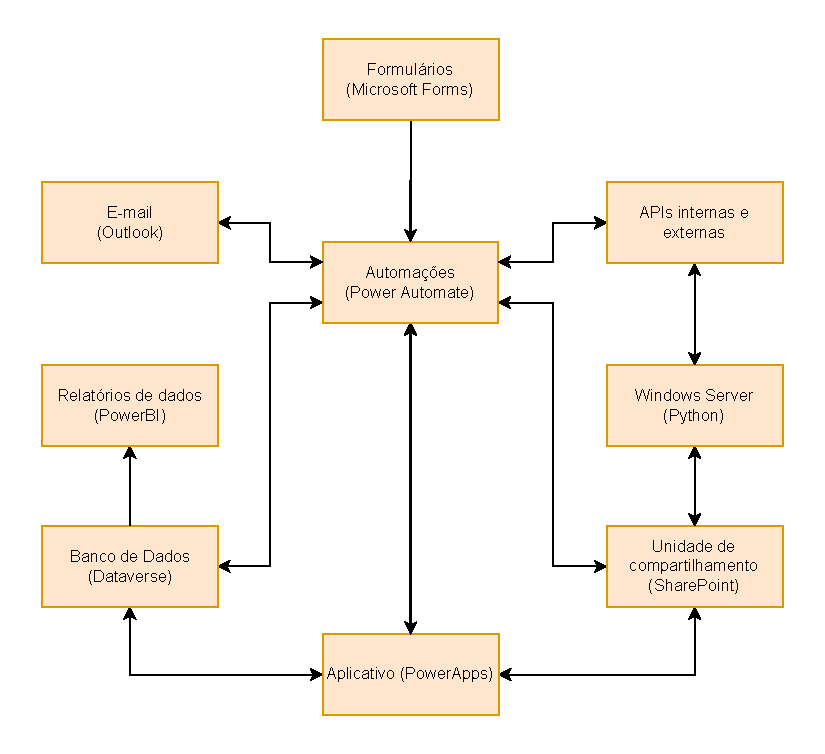
\includegraphics[width=1\textwidth]{./figuras/arquiteturaFisica.pdf}
		\caption{Padrão de arquitetura física dos sistemas desenvolvidos.}
		\label{fig:metodologia:arquiteturaFisica}
	\end{figure}

	Já na figura \ref{fig:metodologia:arquiteturaFuncional} temos o padrão de arquitetura funcional para os sistemas desenvolvidos, e mais uma vez, contém todas as possibilidades
	de funções disponíveis e que podem ser implementadas no sistema de interesse.
	\begin{figure}[h]
		\centering
		% \includegraphics[width=1\textwidth]{./figuras/scattering.eps}
		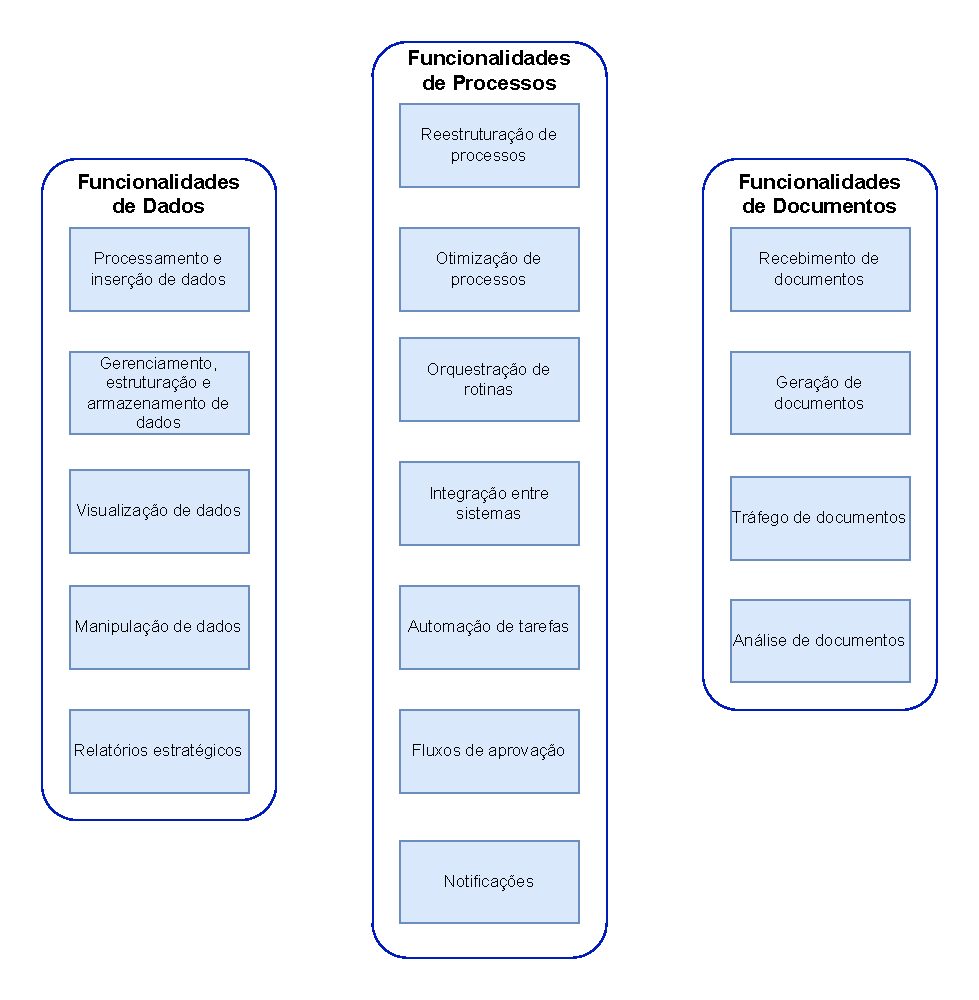
\includegraphics[width=1\textwidth]{./figuras/arquiteturaFuncional.pdf}
		\caption{Padrão de arquitetura funcional dos sistemas desenvolvidos.}
		\label{fig:metodologia:arquiteturaFuncional}
	\end{figure}